\documentclass[sigconf]{acmart}

\usepackage[english]{babel}
\usepackage{blindtext}

% Copyright
\renewcommand\footnotetextcopyrightpermission[1]{} % removes footnote with conference info
\setcopyright{none}
%\setcopyright{acmcopyright}
%\setcopyright{acmlicensed}
%\setcopyright{rightsretained}
%\setcopyright{usgov}
%\setcopyright{usgovmixed}
%\setcopyright{cagov}
%\setcopyright{cagovmixed}

\settopmatter{printacmref=false, printccs=false, printfolios=true}

% DOI
\acmDOI{}

% ISBN
\acmISBN{}

%% {} with no args suppresses printing of the price
\acmPrice{}


\begin{document}
\title{A lightweight python based cluster and workload manager}

%\titlenote{Produces the permission block, and copyright information}
%\subtitle{Extended Abstract}

\author{Ali Hassani}

% The default list of authors is too long for headers}
\renewcommand{\shortauthors}{Hassani}

\begin{abstract}
    Cluster managers are among the key software components in compute clusters.
    They provide an interface to administrators to manage compute nodes, their resources and software, and allow real-time
    monitoring of both physical and logical states. Workload managers on the other hand provide an interface to the users by
    allowing allocating available resources for user-defined compute jobs.
    The goal is to allow users to somewhat abstract their computations from physical nodes by defining jobs on a single ``head''
    node, which, once scheduled, will be distributed among requested resources.
    Herein we present an open source cluster and workload manager written in Python with minimal dependencies, set up to use
    containerization as a means to create virtual nodes within the same physical node.
    Among its applications are partitioning physical resources within one physical node (CPU cores, memory, GPUs) into virtual
    nodes mimicking a compute cluster, and creating an easy and lightweight solution for running and testing 
    parallel/distributed jobs on minimal hardware.
\end{abstract}

\maketitle

\section{Introduction}

Compute clusters are often comprised of a set of networked computers, each with certain computational capabilities and 
resources, and they are set up in such a way that multiple users can request said resources for specific experiments or jobs.
This is a distributed environment, where compute nodes collaborate to create a single unified system through which
researchers, engineers, and scientists conduct computationally heavy experiments based on their requirements, and without having
to consider per-node physical hardware requirements.
An example of that is in machine learning research, where experiments, depending on their nature and size, require different
levels of resources, particularly hardware accelerators, such as general-purpose graphical processing units (GPGPUs) and tensor
processing units (TPUs).
A standard practice in such scenarios is a cluster management software that is installed on all of the networked computers, or
\textit{compute nodes}, and one or more computers manage, organize, and control the rest via network communications made through
the cluster manager, which are referred to as \textit{head nodes}.
Cluster management software relies on a workload management service or module, which provides an interface for users in
order to allow them to request resources, and schedule their jobs accordingly.

SLURM (Simple Linux Utility for Resource Management)~\cite{yoo2003slurm} is one such service, and is among the most widely 
adopted among large-scale supercomputers and compute clusters.
While the cluster management software keeps track of all nodes, their health status, and so on, it also passes their IP 
addresses to the workload manager.
The workload manager, in this case SLURM, runs daemons, which are processes that start automatically after 
the operating system boots and continue to run in background, on head and compute nodes.
On compute nodes, the daemon is responsible for reporting node resource availability, running jobs, and other relevant
information to the head node.
On the head node, controller daemons communicate with communicate with compute nodes, which are exposed via their local IP 
address.

Users then log into head nodes, and use the SLURM interface (commands such as `scontrol`, `sinfo`, `srun`, `sbatch`) to check
available nodes and resources, their running jobs, and submit new jobs.
The interface is responsible for communicating with the daemon to schedule jobs and report information.

\section{Background}

\section{Methodology}
\begin{figure}[ht]
    \centering
    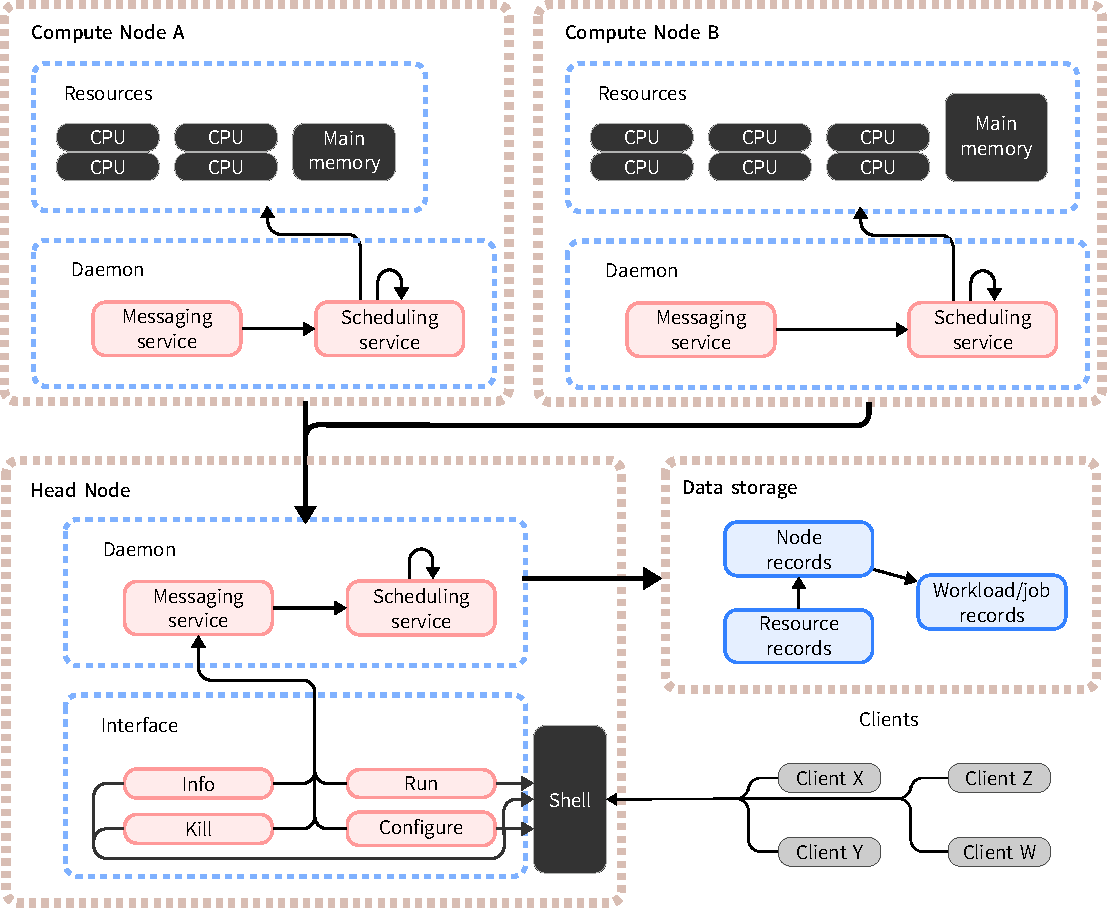
\includegraphics[width=0.475\textwidth]{figures/overview.pdf}
    \caption{
        \textbf{An overview of the components in the proposed cluster manager.}
        Each node will run the CM daemon, which consists of a messaging service, and scheduling service.
        Upon initialization, the daemon is responsible for detecting available resources, starting the services, and registering
        itself with the head node. Head node, once itself initialized, will store information on nodes and resources in a local
        storage. Clients can then use the available interfaces to see available resources, nodes, create/stop jobs, and
        configure the CM (depending on their privileges.)
    }
\end{figure}

\subsection{The First Layer}

\subsection{The Second Layer}

\section{Evaluation}

\section{Conclusion}


\bibliographystyle{acm-reference-format}
\bibliography{references}

\end{document}
